\section{Person Isolation}
\label{person isolation}
\todo{move images to testing}
This section details the creation of a method to isolate a person from the background data. An advantage of using a Kinect over another camera is that the Kinect is able to isolate a skeleton associated with a person. This skeleton meant that the group did not have to make use of computationally heavy computer vision algorithms to isolate a person \todo{example}.\\

Instead, the method developed used the skeleton to determine the approximate depth of the person (using the HipCenter joint). Any point whose depth value is outside a delta (specifically 400) of the HipCenter is discarded. This depth based cut off is illustrated in Figure \ref{fig:depth cut off} below.\\

\begin{figure}[h]
\begin{center}
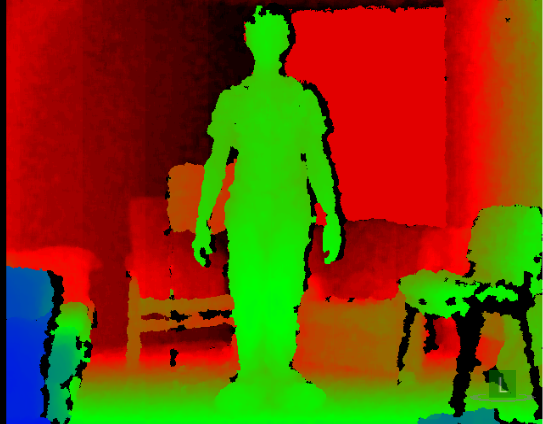
\includegraphics[scale=0.4]{./design/parse1} 
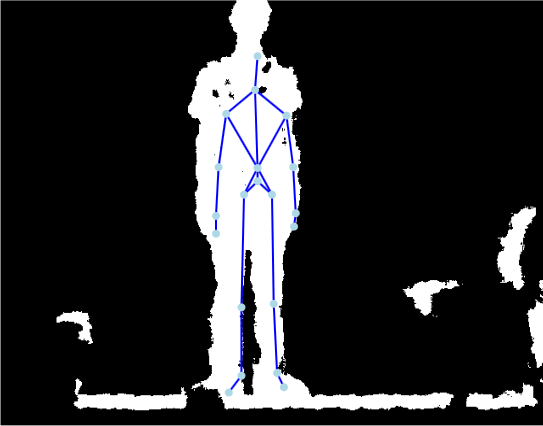
\includegraphics[scale=0.4]{./design/parse2}
\end{center}
\caption{Depth Cut Off, before (left) and after (right).}
\label{fig:depth cut off}
\end{figure} 

Figure \ref{fig:depth cut off} shows that cutting off base depth alone is not enough, as there is a \textit{ring} of equal distant points in-line with the person. To eliminate this ring, the positions of left and right most point of the person (i.e. HandLeft and HandRight) are calculated and anything outside of this range is also discarded. The final result of this can be viewed in Figure \ref{fig:depth and hand cut off}, with the person coloured from black to white as depth increases away from the camera.\\

\begin{figure}[h]
\begin{center}
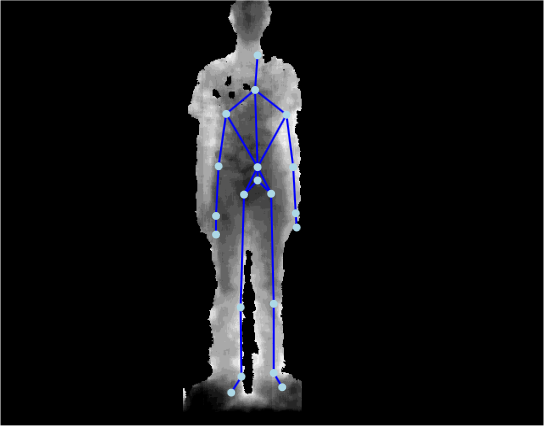
\includegraphics[scale=0.4]{./design/parse3} 
\end{center}
\caption{Depth and Hand Cut Off.}
\label{fig:depth and hand cut off}
\end{figure} 